Docker è un progetto open source con una \href{https://www.docker.com/company}{azienda di supporto che fornisce assistenza} e altri servizi a pagamento per la versione docker-EE. La forza di Docker, e una delle ragioni della sua diffusione, è la sua facilità d’uso. Docker è un insieme di tecnologie che cooperano tra loro al fine di standardizzare il formato dei container e avere un insieme di tool standard e funzionanti che permettono di avere la piena portabilità e poter eseguire i container su diverse piattaforme e host.
Le componenti principali di Docker sono:\\
\begin{figure}[H]
	\begin{center}
		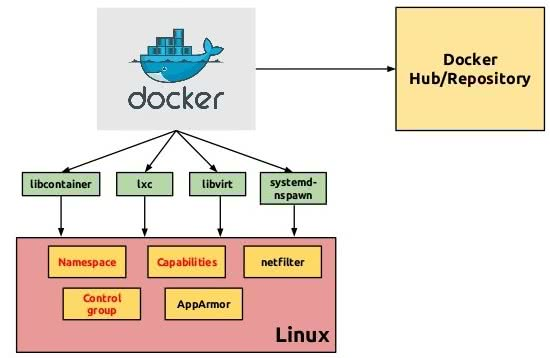
\includegraphics[width=0.99\columnwidth]{img/docker-container_lib.jpg}
		\caption{I registry di Docker.}
		\label{img:API}
	\end{center}
\end{figure}
\begin{itemize}
\item il Docker engine, che è un demone che risiede sul server e accetta comandi da un client (sia da riga di comando sia da chiamate alle API). Esso comunica con il Kernel Linux attraverso la libreria libcontainer (che viene installata insieme a docker).\\
\item il registry, che è una piattaforma che risiede nel cloud e che fornisce un’area dove caricare, scaricare e condividere le immagini dei vari container. Quella ufficiale è \href{https://hub.docker.com/}{https://hub.docker.com}. Supponiamo di voler utilizzare un container con una determinata immagine. Grazie a queste due componenti il cliente chiede al server di prendere quella immagine e “iniettarla” in un container. Il server, se non possiede ancora l’immagine richiesta, contatta il registry. Se esiste nel cloud la scarica e viene creata una copia cache locale. Dopo la inietta in un container. Vedi figura: \ref{img:structDoc1} \ref{img:structDoc2}.\\
\end{itemize}
\begin{figure}[H]
	\begin{center}
		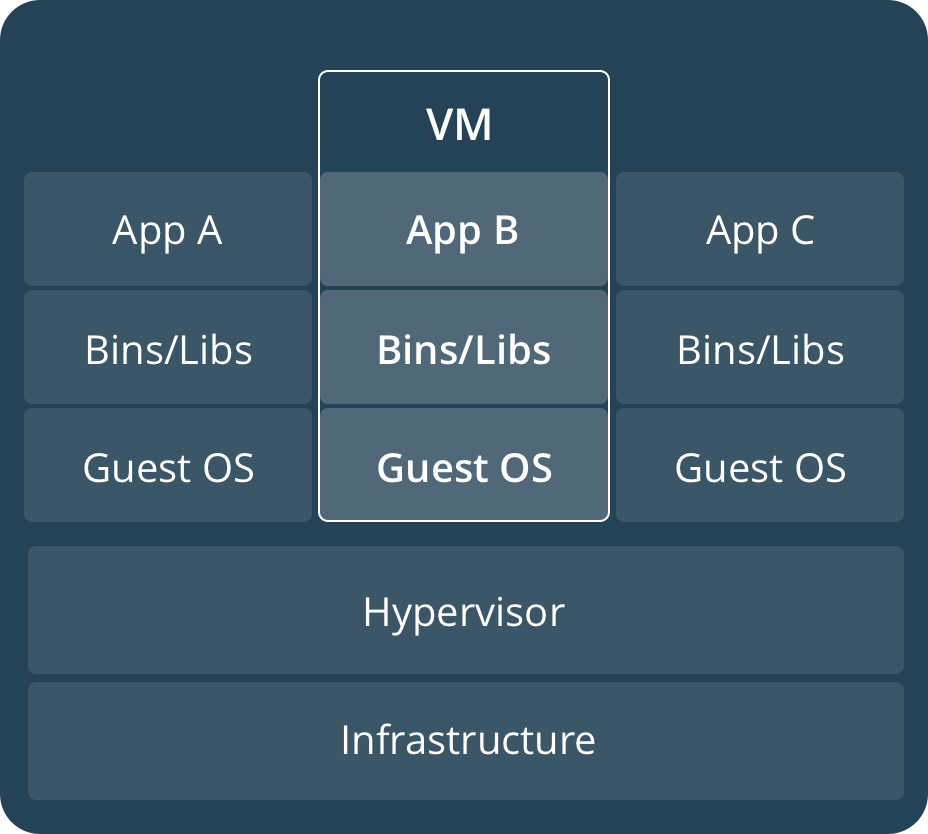
\includegraphics[width=0.70\columnwidth]{img/VM@2x.png}
		\caption{Solution stack classico.}
		\label{img:structDoc1}
	\end{center}
\end{figure}
\begin{figure}[H]
	\begin{center}
		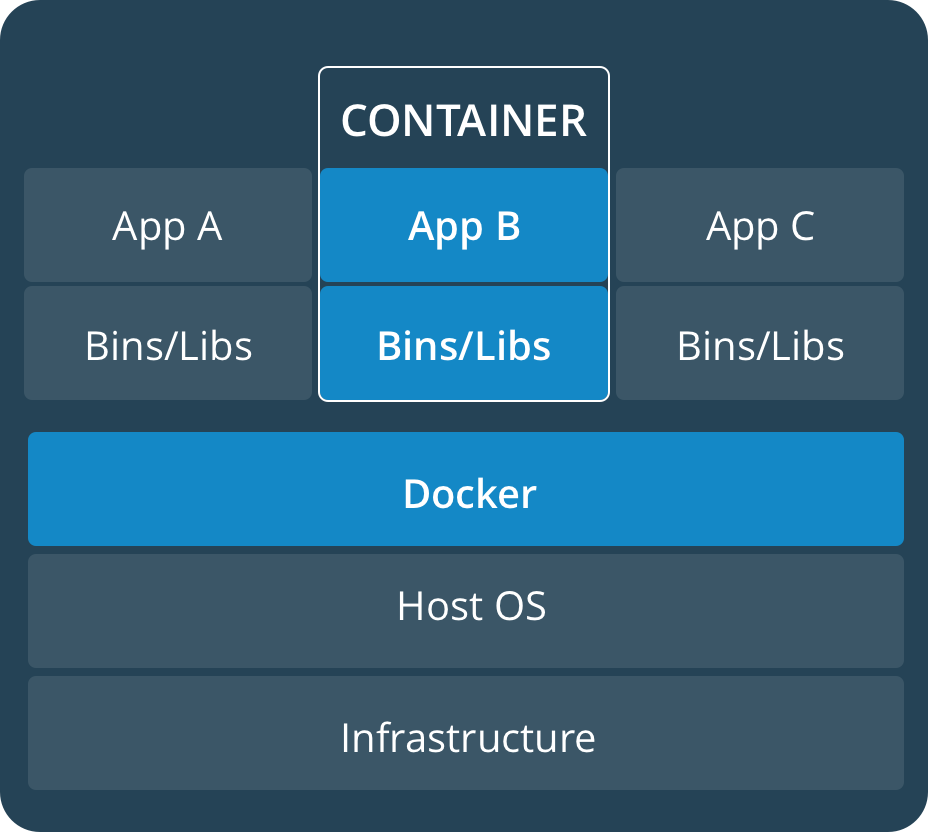
\includegraphics[width=0.70\columnwidth]{img/Container@2x.png}
		\caption{Solution stack di Docker.}
		\label{img:structDoc2}
	\end{center}
\end{figure}
Docker implementa una architettura client–server. Il client è un semplice strumento a linea di comando che invia comandi al server utilizzando servizi REST: questo implica che chiunque potrebbe costruire client differenti. Il server è un daemon Linux in grado di costruire immagini ed eseguire container sulla base di una immagine preesistente.\\Vedi figura: \ref{img:API} \ref{img:registry}
\begin{figure}[H]
	\begin{center}
		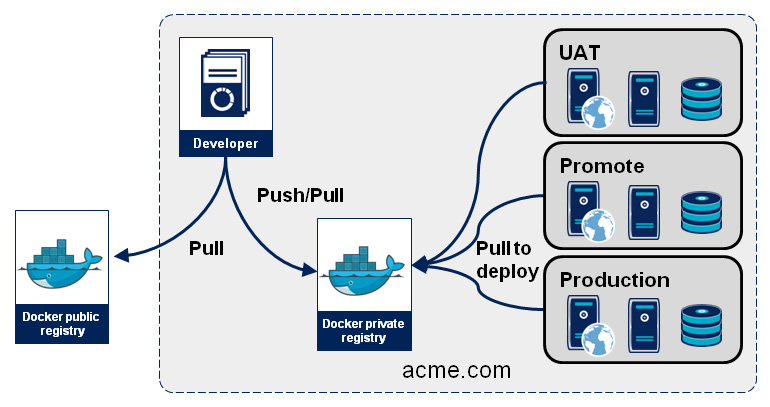
\includegraphics[width=0.99\columnwidth]{img/ContainersOperations-2_fig01.jpg}
		\caption{I registry di Docker.}
		\label{img:registry}
	\end{center}
\end{figure}


